\subsection{Systematic uncertainties}\label{sec:WBoson_Analysis_Systematics}

This section presents the different sources and the procedure employed to determine the systematic uncertainties in the measurement of the \Wb-boson production in \RunpPb collisions. 

%%------------------------------------------------------------%%
\subsubsection{Luminosity}

The recorded integrated luminosity of the 2016 \RunpPb data sample is 173.4~\nbinv, and is known with a precision of 3.5\%~\cite{LUM-17-002}. Since the integrated luminosity cancels in forward-backward ratios and in the muon charge asymmetry, it only affects the measurement of the \WToMuNu differential cross sections. In this case, this 3.5\% systematic uncertainty is global and the bin-to-bin correlation is 100\%. This uncertainty is the dominant one on the \WToMuNu differential cross sections.


%%------------------------------------------------------------%%
\subsubsection{Signal efficiency}

The dominant systematic uncertainties on the forward-backward ratios and muon charge asymmetry are due to the estimation of the signal efficiency. Since the signal efficiencies are computed from simulations and corrected using the \tnp corrections, two sources of systematic uncertainties are considered. The first one corresponds to the theoretical modelling of the simulated signal, which takes into account the uncertainty on the nuclear PDFs and the impact of the renormalisation and factorisation scales. The second source corresponds to the \tnp correction uncertainties, which derive from the \ZToMuMu control sample used to extract the \tnp data efficiencies.

\paragraph{Theoretical modelling.} The NLO model used to generate the simulations can impact the measurement of the signal efficiencies. The main sources of theoretical uncertainties include the choice of the nuclear parton distribution functions (EPPS16+CT14), and the renormalisation and factorisation scales.

Since the PDFs are not calculable from first principles but are determined experimentally, in particular by the measurements reported here, the inclusion of any PDF introduces an additional systematic uncertainty. Thus, it is important to determine the impact of a change of PDF on the signal efficiencies. The procedure to derive the theoretical uncertainties of the PDF variations consists of reweighing the simulations event-by-event using weights derived from \POWHEG after applying various PDF sets. The PDF sets are accessed through the LHAPDF6~\cite{LHAPDF6} framework and consist of 56 CT14 PDFs and 40 EPPS16 nuclear corrections. Once the simulations are reweighed with each PDF set, the efficiencies are recomputed and used to recalculate all the observables. The nPDF uncertainty is determined by combining the EPPS16+CT14 PDF variations of the observables using the Hessian approach, as recommended by the EPPS16 authors~\cite{EPPS16}. 

Moreover, the uncertainty due to the renormalisation ($\mu_{R}$) and factorisation ($\mu_{F}$) scales is computed by varying these two scales in \POWHEG using the following six combinations:
\begin{equation*}
\left(\frac{\mu_{R}}{M_{\PW}} , \frac{\mu_{F}}{M_{\PW}}\right) = [\ (0.5 , 0.5)\ ,\ (1.0 , 0.5)\ ,\ (0.5 , 1.0)\ ,\ (1.0 , 2.0)\ ,\ (2.0 , 1.0)\ ,\ (2.0 , 2.0)\ ]
\end{equation*}

The simulations are reweighed event-by-event using the \POWHEG weights produced with each set of scales, then the efficiencies are recomputed and the observables are recalculated for each varied efficiency. The variations on the observables are combined by taking the envelope (i.e. the maximum variation in each \etaMuCM range).

The systematic uncertainties from the PDF and scale variations are summed in quadrature, and amount to 0.1\%. Thus, the theoretical uncertainties have negligible impact on the signal efficiencies.

\paragraph{Tag-and-probe corrections.} The main source of systematic uncertainty in the measurement of the signal efficiency arises from the application of the \tnp corrections. As mentioned in \sect{sec:WBoson_Analysis_Efficiency_Corrected}, the statistical and systematic uncertainties of the \tnp corrections are derived from the muon identification, isolation and trigger efficiencies measured in data.

It is crucial to consider the correlation between the different \tnp uncertainties as a function of muon pseudorapidity and its charge, since they could cancel in the forward-backward ratios and muon charge asymmetry. The statistical \tnp variations are uncorrelated between the different \etaLAB ranges in which they were derived. The systematic \tnp variations are considered to be fully correlated as a function of muon charge since the detector response is the same for muons and anti-muons, and uncorrelated between the different \etaCM ranges (spanning different detectors).

To compute the uncertainties, the muon charge asymmetry and the forward-backward ratios are recalculated for each efficiency derived by varying the \tnp corrections. The \tnp uncertainties are then determined by taking the difference between the value obtained with the varied \tnp correction and its nominal value, combining the uncertainties as explained in \sect{sec:WBoson_Analysis_Efficiency_Corrected}. If the source of \tnp correction is correlated in muon charge or pseudorapidity, the corresponding signal yields are varied at the same time. Moreover, for the \Wpm differential cross sections, the statistical and systematic \tnp uncertainties are calculated by propagating the uncertainties on the corrected signal efficiency.

The largest systematic uncertainty due to the \tnp corrections amounts to 3.2\% and the dominant \tnp uncertainties are derived from the \tnp systematic variations of the muon isolation (2.5\%) and trigger (1.1\%) components. The \tnp systematic uncertainties on the muon isolation and trigger efficiency mainly arise from varying the background functional form used to fit the tag-probe invariant mass distribution, which lacks of statistics.

%%------------------------------------------------------------%%
\subsubsection{QCD jet background}

The systematic uncertainty in the QCD jet background originates from the uncertainty in the modelling of the QCD jet \ptmiss distribution in the signal region. The nominal procedure consists in fixing the parameters of the modified Rayleigh distribution from the fits extrapolated from data as explained in \sect{sec:WBoson_Analysis_SignalExtraction_QCDBackground}. In order to estimate the uncertainty of the mismodelling of the \ptmiss distribution of the QCD jet background, both the parameters and the functional form are varied.

\paragraph{QCD jet background parameters.} The first source of systematic uncertainty reflects the possible mismodelling of the QCD jet background shape due to the \etaMuCM dependence of the QCD background parameters. In order to check this, the parameters of the nominal QCD jet model are set free but constrained to be near their nominal values by using a Gaussian penalty. The width of the penalty Gaussian function is fixed, for a given QCD background parameter, to the root mean square (RMS) of the set of extrapolated results along all \etaMuCM ranges, shown in \fig{fig:QCD_Extrapolation_Eta}. The RMS values used in the Gaussian penalty for the $\sigma_{0}$,  $\sigma_{1}$ and  $\sigma_{2}$ parameters are presented in \tab{tab:QCDContrainPar}. The difference between the number of signal events extracted from the Gaussian-constrained fits and the nominal fits is taken as the systematic uncertainty, which is then propagated to all observables. This source of uncertainty is considered to be fully uncorrelated since the \ptmiss distribution in each \etaMuCM range is fitted separately.

\begin{table}[htb!]
  \centering
  \begin{tabular}{|c|c c|}\hline
  \multirow{2}{*}{Parameter} & \multicolumn{2}{c|}{RMS} \\
   & $\text{QCD jet} \to \mu^{-}$ & $\text{QCD jet} \to \mu^{+}$ \\\hline
  $\sigma_{0}$ & 1.0 & 0.5 \\\hline
  $\sigma_{1}$ & 0.9 & 0.9\\\hline
  $\sigma_{2}$ & 0.7 & 0.6\\\hline
  \end{tabular}
  \caption{The RMS of the set of QCD background parameters extrapolated along all \etaMuCM regions.}
  \label{tab:QCDContrainPar}
\end{table}

Another systematic variation consists of changing the muon isolation point used to extrapolate the QCD background parameters. In the nominal case, the isolation point of 0.03 is determined from the average muon isolation value in data within the signal region. As an alternative case, the muon isolation distribution is checked in a QCD \PYTHIA simulated sample satisfying the signal selection criteria, and the average isolation value is determined to be approximately 0.08. As a result, the QCD background parameters are recomputed by extrapolating them to an isolation point of $\iso=0.08$, and the fits are redone by fixing the QCD background parameters to the extrapolated values in the \etaMuCM-inclusive range as in the nominal case. The difference between the number of signal events extracted from the fits using the varied QCD background shape and the nominal results is taken as the systematic uncertainty. This uncertainty is propagated to all observables. The QCD background parameters extrapolated to $\iso=0.08$ are listed in \tab{tab:QCDFixedPar_Iso0p08}. Since the result in each \etaMuCM range varies independently, the uncertainty is considered to be fully uncorrelated.

\begin{table}[htb!]
  \centering
  \begin{tabular}{|c|c|c|}\hline
   Parameter & $QCD \to \mu^{-}$ & $QCD \to \mu^{+}$ \\\hline
   $\sigma_{0}$ & 14.67 & 14.79 \\\hline
   $\sigma_{1}$ & 6.28 & 6.71 \\\hline
   $\sigma_{2}$ & 0.50 & 0.49 \\\hline
  \end{tabular}
  \caption{QCD shape parameters extrapolated to the average muon isolation point $\iso = 0.08$.}
  \label{tab:QCDFixedPar_Iso0p08}
\end{table}

The systematic uncertainty associated to the \etaMuCM dependence of the QCD background parameters amounts to 1.1\%, while the uncertainty corresponding to the change of extrapolation point represents 0.2\%.

\paragraph{QCD jet background functional form.} To assign a systematic uncertainty due to the assumed functional form for modelling the QCD jet background \ptmiss distribution, a different model is used. The alternative \ptmiss functional form employed, taken from Ref.\cite{HIN-13-007}, is given by: 

\begin{equation}\label{eq:QCDMultiJet}
  f_{\text{QCD}}\left(\ptmiss\right) = \left(\ptmiss+x_0\right)^{\alpha}\cdot\exp\left(\beta\cdot\sqrt{\ptmiss+x_0}\right)
\end{equation}

The extrapolation procedure explained in \sect{sec:WBoson_Analysis_SignalExtraction_QCDBackground} is redone using the alternative model. All the fits are remade using the alternative QCD background functional form fixed to the parameters extrapolated in the \etaMuCM-inclusive range. The difference between the number of signal events measured using the alternative QCD background model and the nominal results is taken as the systematic uncertainty due to mismodelling of the QCD jet background shape. This systematic uncertainty is propagated to all observables and amounts to 0.6\%. The bin-to-bin correlation is taken to be fully uncorrelated.

%%------------------------------------------------------------%%
\subsubsection{Electroweak and \ttbar backgrounds}

The \ttbar background and the different sources of electroweak background are described using template histograms derived from simulations. The simulated samples are scaled to the recorded integrated luminosity of data using the NLO \POWHEG cross sections for the electroweak processes and the CMS measured cross section for the \ttbar production. Since for each these background sources, the ratio of background over signal events is fixed to simulation when performing the fits, a systematic uncertainty is assigned to each source by varying up and down their cross sections as explained below. The systematic uncertainty in each \etaMuCM range is derived by taking the maximum difference between the nominal and the up/down variations. The bin-to-bin correlations in muon charge and pseudorapidity are considered correlated since the total cross section is used to normalise all simulated events.

\paragraph{\texorpdfstring{\DYToMuMu}\ background.} The uncertainty on the ratio of $\Z/\Wb$ total cross sections is estimated using the Monte Carlo for FeMtobarn processes (MCFM) program~\cite{MCFM} at NLO with the CT14+EPPS16 nuclear PDFs. A relative uncertainty of $0.8\%$ for $Z/\Wm$ and $1.3\%$ for $Z/\Wp$ cross-section ratios is determined with MCFM taking into account the PDF uncertainties. Since the cross sections in the muon channel depend on the branching ratio associated to each process, their uncertainty has to also be taken into account. The values of the branching ratios correspond to $\textrm{BR}(\ZToMuMu) = (3.366 \pm 0.007)\%$ and $\textrm{BR}(\WToMuNu) = (10.63 \pm 0.15)\%$~\cite{PDG}, which gives a relative uncertainty on the ratio of $\Z/\Wb$ branching ratios of $1.4\%$. Summing in quadrature the MCFM uncertainties with the ones derived from the branching ratios, one gets a total relative uncertainty for $\Z/\Wp$ of $1.6\%$ and for $\Z/\Wm$ of $1.9\%$. To be conservative the systematic variation is fixed to $2\%$ overall. The systematic uncertainty on the \PW-boson yield is then determined by varying the \DYToMuMu cross section by $2\%$ up and down when performing the fits, yielding a change of 0.3\% in the measured \WToMuNu cross sections.

\paragraph{\texorpdfstring{\DYToTauTau}\ background.} The uncertainty on the ratio of \DYToTauTau background over signal events is considered to be the same as the 2\% uncertainty determined for the \DYToMuMu background. Hence, the \DYToTauTau cross section is varied by $2\%$ up and down when performing the fits. The impact of this systematic uncertainty is negligible and modifies the \WToMuNu cross sections by 0.01\%.

\paragraph{\texorpdfstring{\WToTauNu}\ background.} The values of the \Wb-boson leptonic branching ratios correspond to $\textrm{BR}(\WToMuNu) = (10.63 \pm 0.15)\%$ and $\textrm{BR}(\WToTauNu) = (11.38 \pm 0.21)\%$~\cite{PDG}, which gives a relative uncertainty on the ratio of \WToTauNu over \WToMuNu cross sections of $2.3\%$. Thus, the systematic uncertainty is estimated by varying the ratio of \WToTauNu to signal events up and down by $\pm$2.3\%. The impact of this systematic uncertainty on the \WToMuNu cross sections is found to be 0.04\%.

\paragraph{\texorpdfstring{\ttbar}\ background.} The \ttbar simulation is normalized using the CMS measured total cross section $\sigma_{\ttbar} = 45 \pm 8$~nb~\cite{HIN-17-002}. The systematic related to the \ttbar background normalization is computed by varying up and down the \ttbar cross section by its measured relative uncertainty ($\pm$18\%). This systematic uncertainty amounts to 0.2\%.

%%------------------------------------------------------------%%
\subsubsection{Weak boson \pt}\label{sec:Systematic_BosonPTCorr}

The modelling of the weak boson \pt in the signal and electroweak background simulations is corrected by weighing event-by-event the generated weak boson \pt distribution following the procedure described in \sect{sec:WBoson_Analysis_Corrections_WeakBosonPTReweighing}. To determine the impact of the modelling of the weak boson \pt, the boson \pt corrections are removed and both the efficiency and the fits to the \ptmiss distribution are remade. The systematic uncertainty is determined in each \etaMuCM range from the difference between the nominal results and the results obtained without weighing the generated boson \pt distribution. This uncertainty amounts to 0.5\% and it is considered to be correlated with respect to muon charge and pseudorapidity.

%%------------------------------------------------------------%%
\subsubsection{Event activity}\label{sec:WBoson_Analysis_Systematics_EventActivity}

The modelling of the event activity present in \RunpPb collisions is improved by weighing the distribution of the total HF energy, as explained in \sect{sec:WBoson_Analysis_Corrections_EventActivityReweighing}. The event activity is also correlated with other global variables, such as the number of tracks per event.
Since the pseudorapidity coverages of the tracker ($|\eta| < 2.5$) and the HF calorimeter ($3.0 < |\eta| < 5.4$) are different, the HF energy and the track multiplicity are sensitive to different kinematic regions of the event activity. Thus, the systematic uncertainty on the modelling of the event activity is determined by weighing instead the distribution of the simulated track multiplicity following the same procedure as the one used for the HF energy. The fits to the \ptmiss distribution and the signal efficiency are recomputed after weighing the simulated track multiplicity distribution. The difference between the varied and nominal observables is assigned as the systematic uncertainty in each muon \etaMuCM range. This uncertainty is considered correlated in muon charge and pseudorapidity, and it amounts to 0.6\%.

%%------------------------------------------------------------%%
\subsubsection{Recoil calibration}

The uncertainties due to the recoil calibration are of different nature: statistical and systematic. The statistical component arises from the uncertainties associated to the recoil scale and resolution derived from the fits to the recoil distributions from data. The systematic components arise from the following sources:
\begin{itemize}
 \item The recoil calibration method employed to correct the simulated \ptmiss distribution;
 \item The choice of functional form used to fit the recoil distributions in each \qtZ range;
 \item The parametrisation of the \qt dependence of the recoil scale and resolution.
\end{itemize}

\paragraph{Statistical component.} In order to estimate the uncertainty associated to the recoil resolution, the weighed average Gaussian widths of the perpendicular and parallel recoil components, defined in \eq{eq:SigmaAvg}, are randomly smeared in each \qtZ range using a Gaussian distribution centred on the parameter value and with a width equal to the parameter uncertainty. The \qt dependence is parametrised again using the nominal functions presented in \eq{eq:equreolnparam}. The procedure is repeated a hundred times, and the recoil calibrations are applied to the simulated \ptmiss distributions, redoing the measurements every time. The RMS of the number of signal events extracted from the fits using each variation of the recoil calibration, is used to determine the statistical uncertainty of the recoil calibration. This uncertainty is propagated to all observables and amounts to 0.09\%. It is considered fully uncorrelated.

\paragraph{Systematic components.} The fit function used to parametrise the \qt dependence of the recoil scale and resolution, is varied in both data and simulation to determine the associated uncertainty. Instead of using the nominal functions for the Gaussian mean (\eq{eq:equparparam}) and Gaussian widths (\eq{eq:equreolnparam}), a second order polynomial is used to parametrise the Gaussian parameters with respect to \qtZ. The varied recoil calibration is applied to the simulated \ptmiss distributions, which are then used to extract the signal from the data. The difference between the observables measured using the varied recoil calibration and the nominal observables, in each \etaMuCM, is assigned as a systematic uncertainty.

The uncertainty on the shape of the recoil distributions in each \qtZ range is estimated by varying the recoil fit model. Instead of using a sum of two Gaussian functions, the recoil distributions are parametrised with a sum of a Breit-Wigner and a Gaussian distribution, in both data and simulation (varied at the same time). The resulting \qt dependence of the recoil scale and resolution is determined following the nominal procedure and the measurements are performed again. The systematic uncertainty is determined as the variation between the observables derived with the varied recoil calibration and the nominal ones.

Moreover, the uncertainty associated to the method used to apply the recoil calibration is determined by smearing the recoil distributions as described in \eq{eq:RecoilCorrAlt}, instead of scaling them as done in the nominal case. The difference between the varied and nominal observables in each \etaMuCM is assigned as a systematic uncertainty.

The largest source of systematic uncertainty in this case is the one associated to the shape of the recoil distribution, which amounts to 0.3\%. The uncertainty related to the recoil calibration represents 0.2\%, while the uncertainty corresponding to the \qt dependence of the recoil scale and resolution is determined to be 0.06\%. These uncertainties are considered correlated both in muon charge and pseudorapidity.

%%------------------------------------------------------------%%
\subsubsection{W-boson POWHEG BOX}

The \WToMuNu simulations were generated using the \POWHEGBOX package \verb#W_ew-BMMNP# \cite{POWHEGBOX_W_ew_BMNNP}, in which electroweak NLO corrections are implemented. In order to assess the impact of these NLO corrections on the final results, the \WToMuNu simulations were remade instead using the standard \POWHEGBOX package \verb#W#~\cite{POWHEGBOX_W}, which does not include electroweak NLO corrections, following the same procedure described in \sect{sec:WBoson_Analysis_Sample_MC}.

To determine the systematic uncertainty, the signal efficiencies and the template histograms for the signal were recomputed using the \WToMuNu simulations without electroweak NLO corrections. Then, the fits to the \ptmiss distribution in data were performed again, and the difference between the observables measured using the varied signal templates and the nominal results is assigned as a systematic uncertainty in each $\etaMuCM$ range. This uncertainty amounts to 0.9\% and it is considered to be fully correlated.

%%------------------------------------------------------------%%
\subsubsection{Summary of systematic uncertainties}

The largest systematic uncertainty for each category among all \etaMuCM ranges is summarised in \tab{tab:Systematics}. The systematic uncertainties are shown for each observable, including the \WToMuNu cross sections, muon charge asymmetry and the forward-backward ratios. The uncertainties presented for the cross sections are relative while those for the forward-backward ratios and the muon charge asymmetry are absolute.

\begin{table}[htb!]
  \centering
  \resizebox{\textwidth}{!}{
  %\renewcommand{\arraystretch}{1.5}
  \begin{tabular}{|c|*6c|}
    \hline
    Systematic Variation & $\sigma\left(\WToMuNuMi\right)$~[$\%$]  & $\sigma\left(\WToMuNuPl\right)$~[$\%$] & $\RFBm$ & $\RFBp$ & $\RFB$ & $\ChgAsym$\\
    \hline
    Luminosity &  3.5  &  3.5  &  0.000  &  0.000  &  0.000  &  0.000 \\
    \hline
    Signal efficiency &  3.0  &  3.2  &  0.026  &  0.037  &  0.030  &  0.011 \\
    \hline
    QCD jet background &  1.2  &  0.7  &  0.016  &  0.007  &  0.009  &  0.006 \\
    \hline
    Electroweak and \ttbar backgrounds &  0.4  &  0.3  &  0.002  &  0.001  &  0.001  &  0.000 \\
    \hline
    Weak boson \pt &  0.5  &  0.4  &  0.001  &  0.001  &  0.001  &  0.001 \\
    \hline
    Event activity &  0.6  &  0.4  &  0.002  &  0.002  &  0.001  &  0.002 \\
    \hline
    Recoil calibration &  0.2  &  0.3  &  0.002  &  0.004  &  0.002  &  0.002 \\
    \hline
    W-boson \POWHEGBOX &  0.9  &  0.5  &  0.007  &  0.004  &  0.006  &  0.003 \\
    \hline
    Total systematic uncertainty &  4.8  &  4.8  &  0.030  &  0.038  &  0.031  &  0.013 \\
    \hline
    Statistical  uncertainty &  2.4  &  2.0  &  0.026  &  0.029  &  0.019  &  0.015 \\
    \hline
  \end{tabular}
  }
  \caption{Maximum uncertainty of the measured observables determined for each category. The uncertainties of the \WToMuNu differential cross sections are relative while for the forward-backward ratios and muon charge asymmetry are absolute.}
  \label{tab:Systematics}
\end{table}




The uncertainties of the measurements are shown in \fig{fig:Summary_Systematics} as a function of \etaMuCM. They are observed to be similar between the different \etaMuCM ranges, except for the most backward and forward regions, which are driven by the systematic uncertainty on the signal efficiency. It is also seen that the systematic uncertainties dominate on the \WToMuNupm differential cross sections and the forward-backward ratios in all \etaMuCM ranges. In the case of the muon charge asymmetry, most of the systematic uncertainties are found to be suppressed due to the correlations in muon charge, and as a result, the statistical uncertainties dominate in most of the \etaMuCM ranges.

\begin{figure}[!htbp]
 \thisfloatpagestyle{empty}
 \centering
 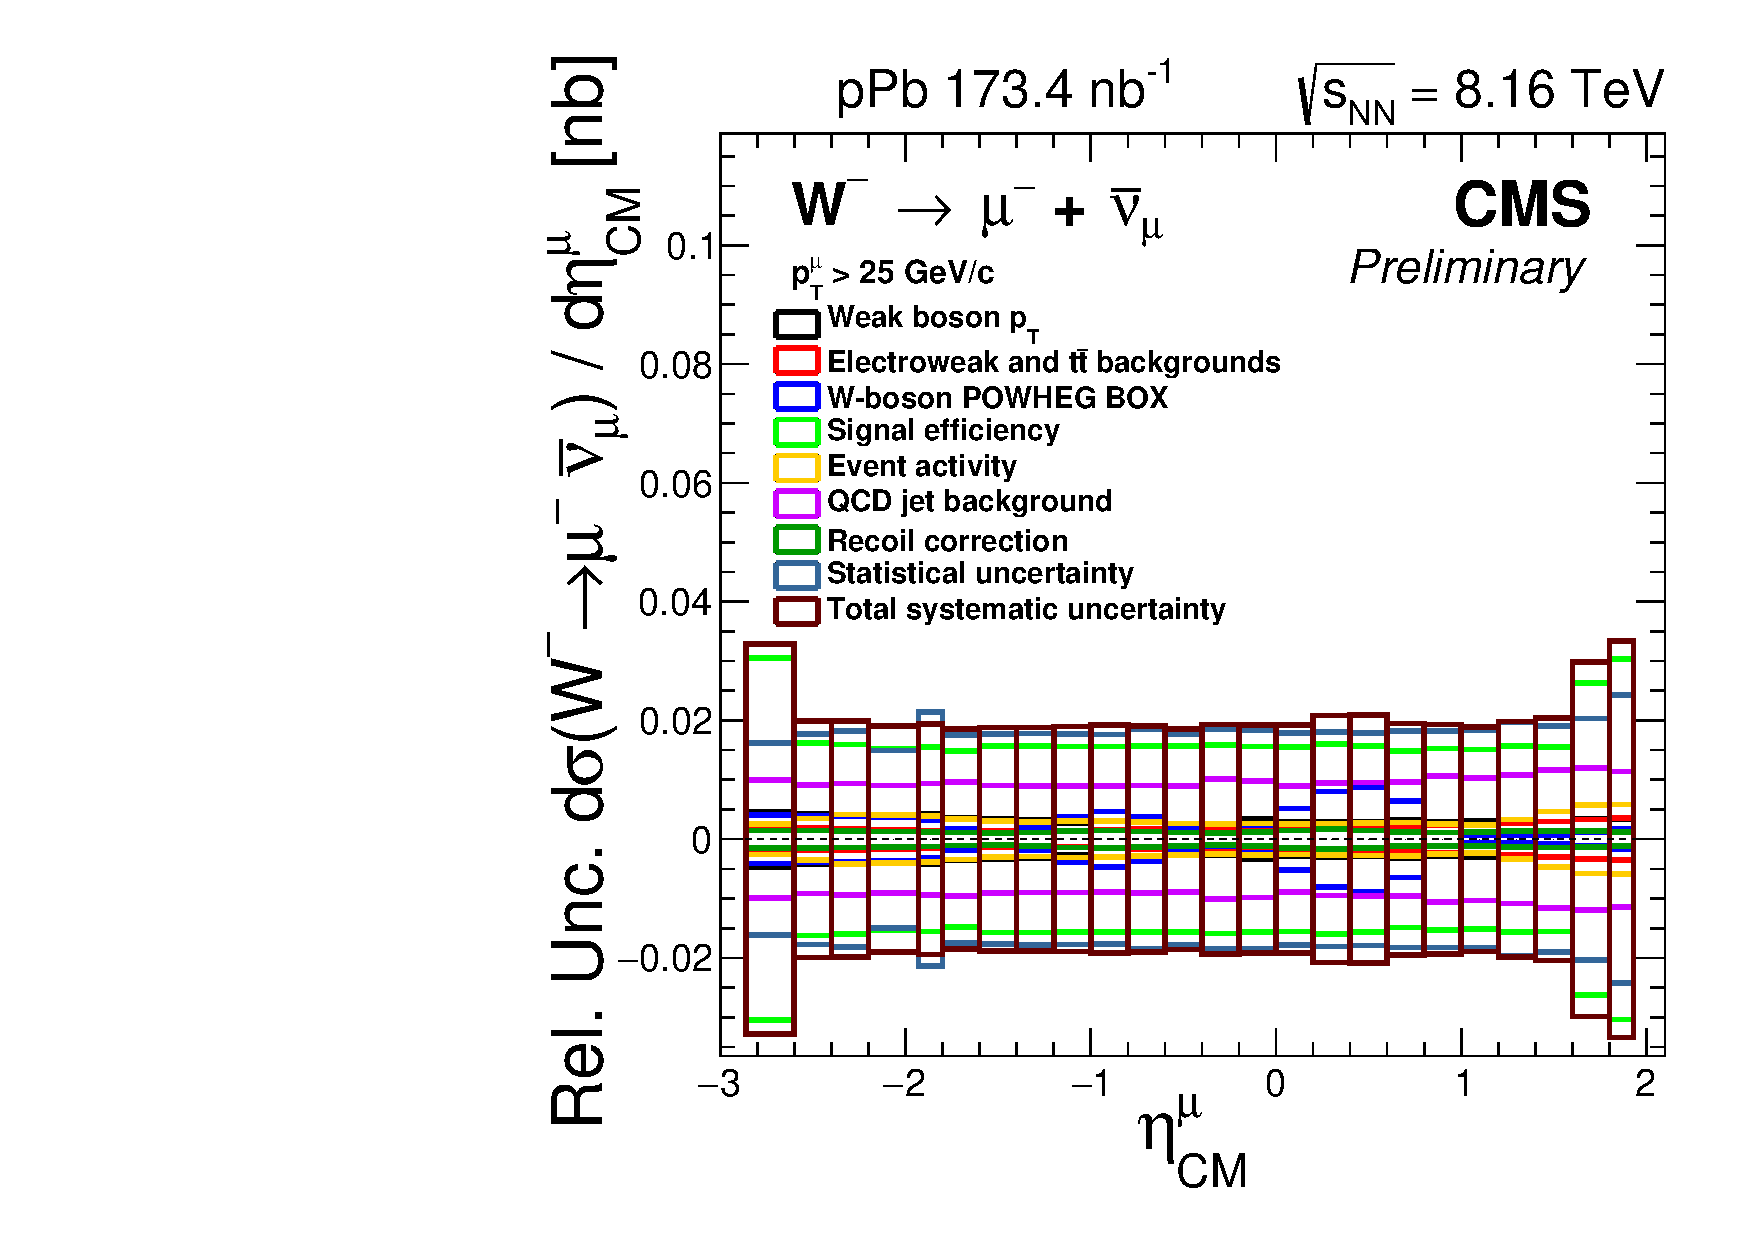
\includegraphics[width=0.45\textwidth]{Figures/WBoson/Analysis/Systematics/gr_WToMuMi_PA_Cross_Section_EffTnP.pdf}
 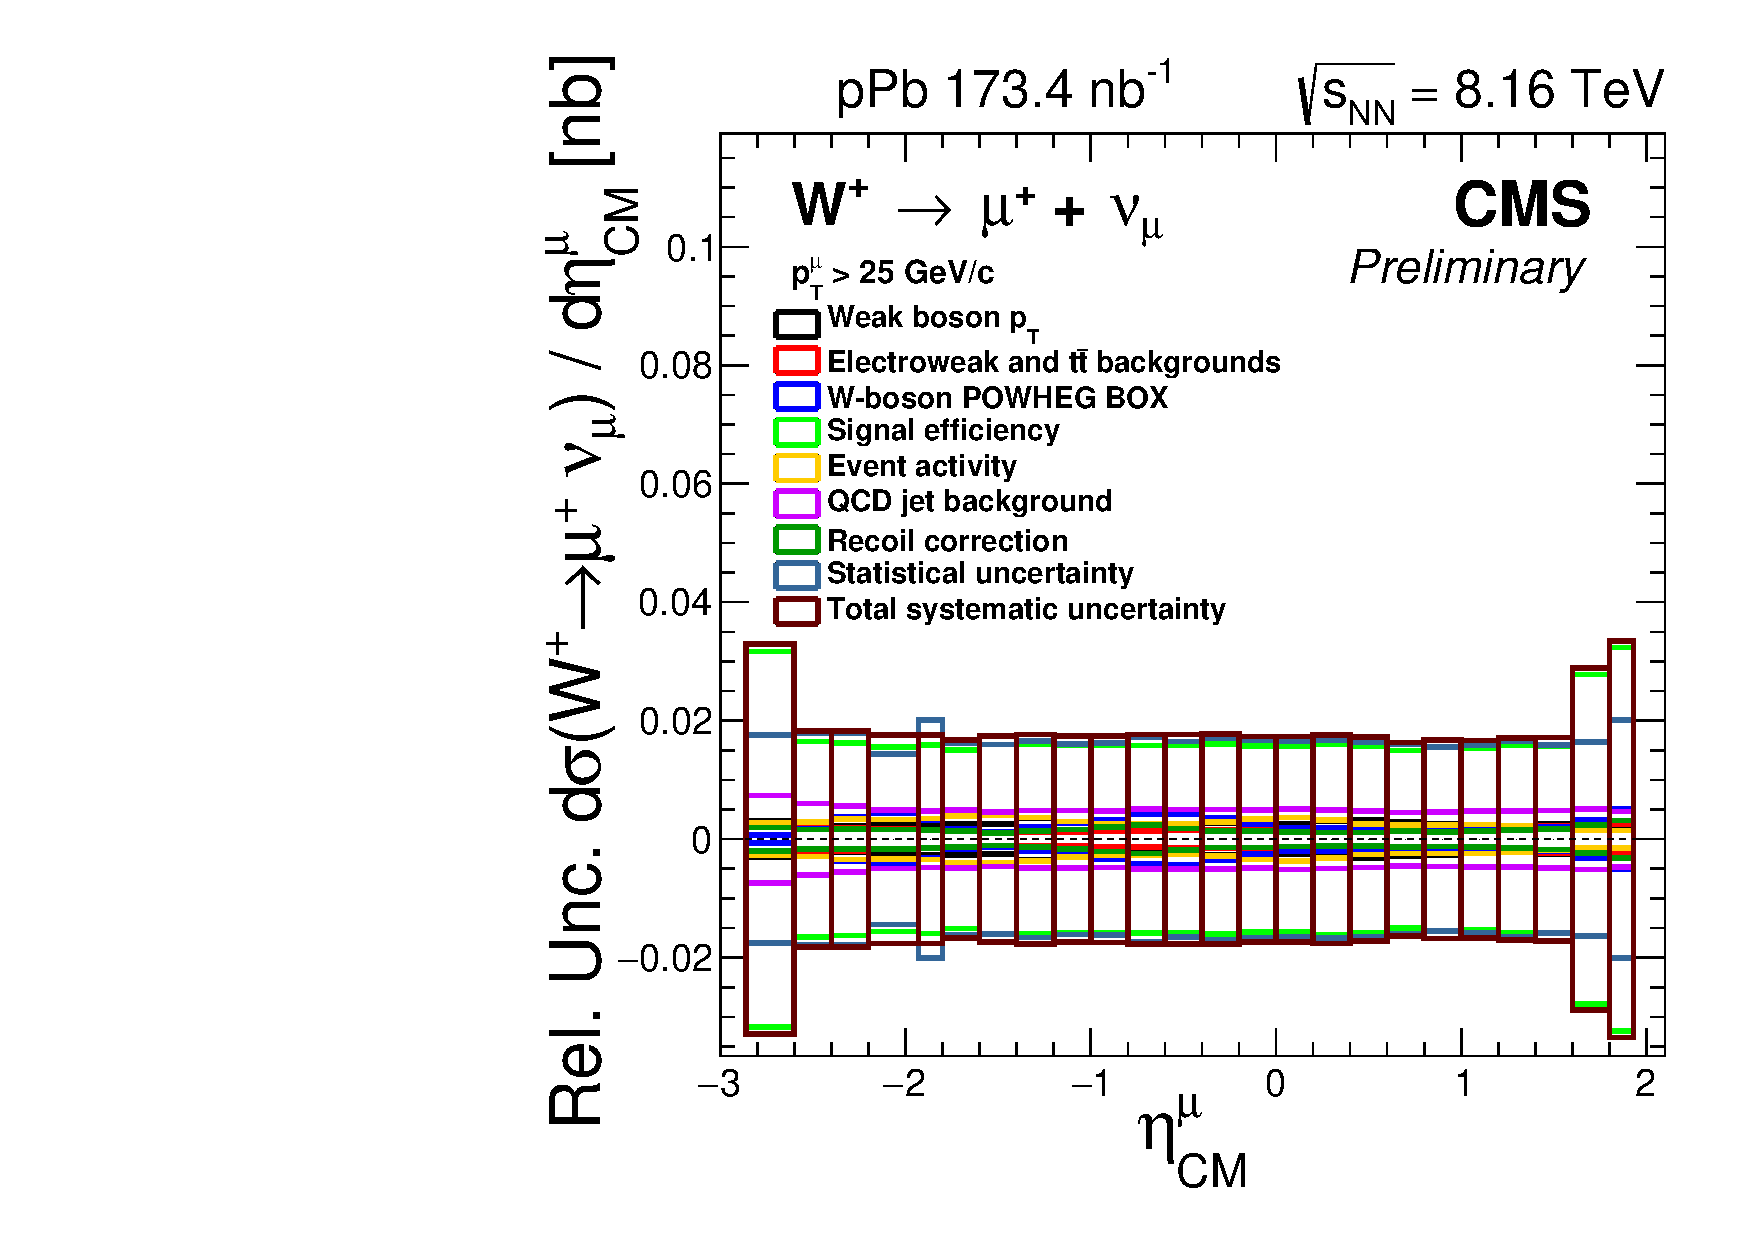
\includegraphics[width=0.45\textwidth]{Figures/WBoson/Analysis/Systematics/gr_WToMuPl_PA_Cross_Section_EffTnP.pdf}
\\
 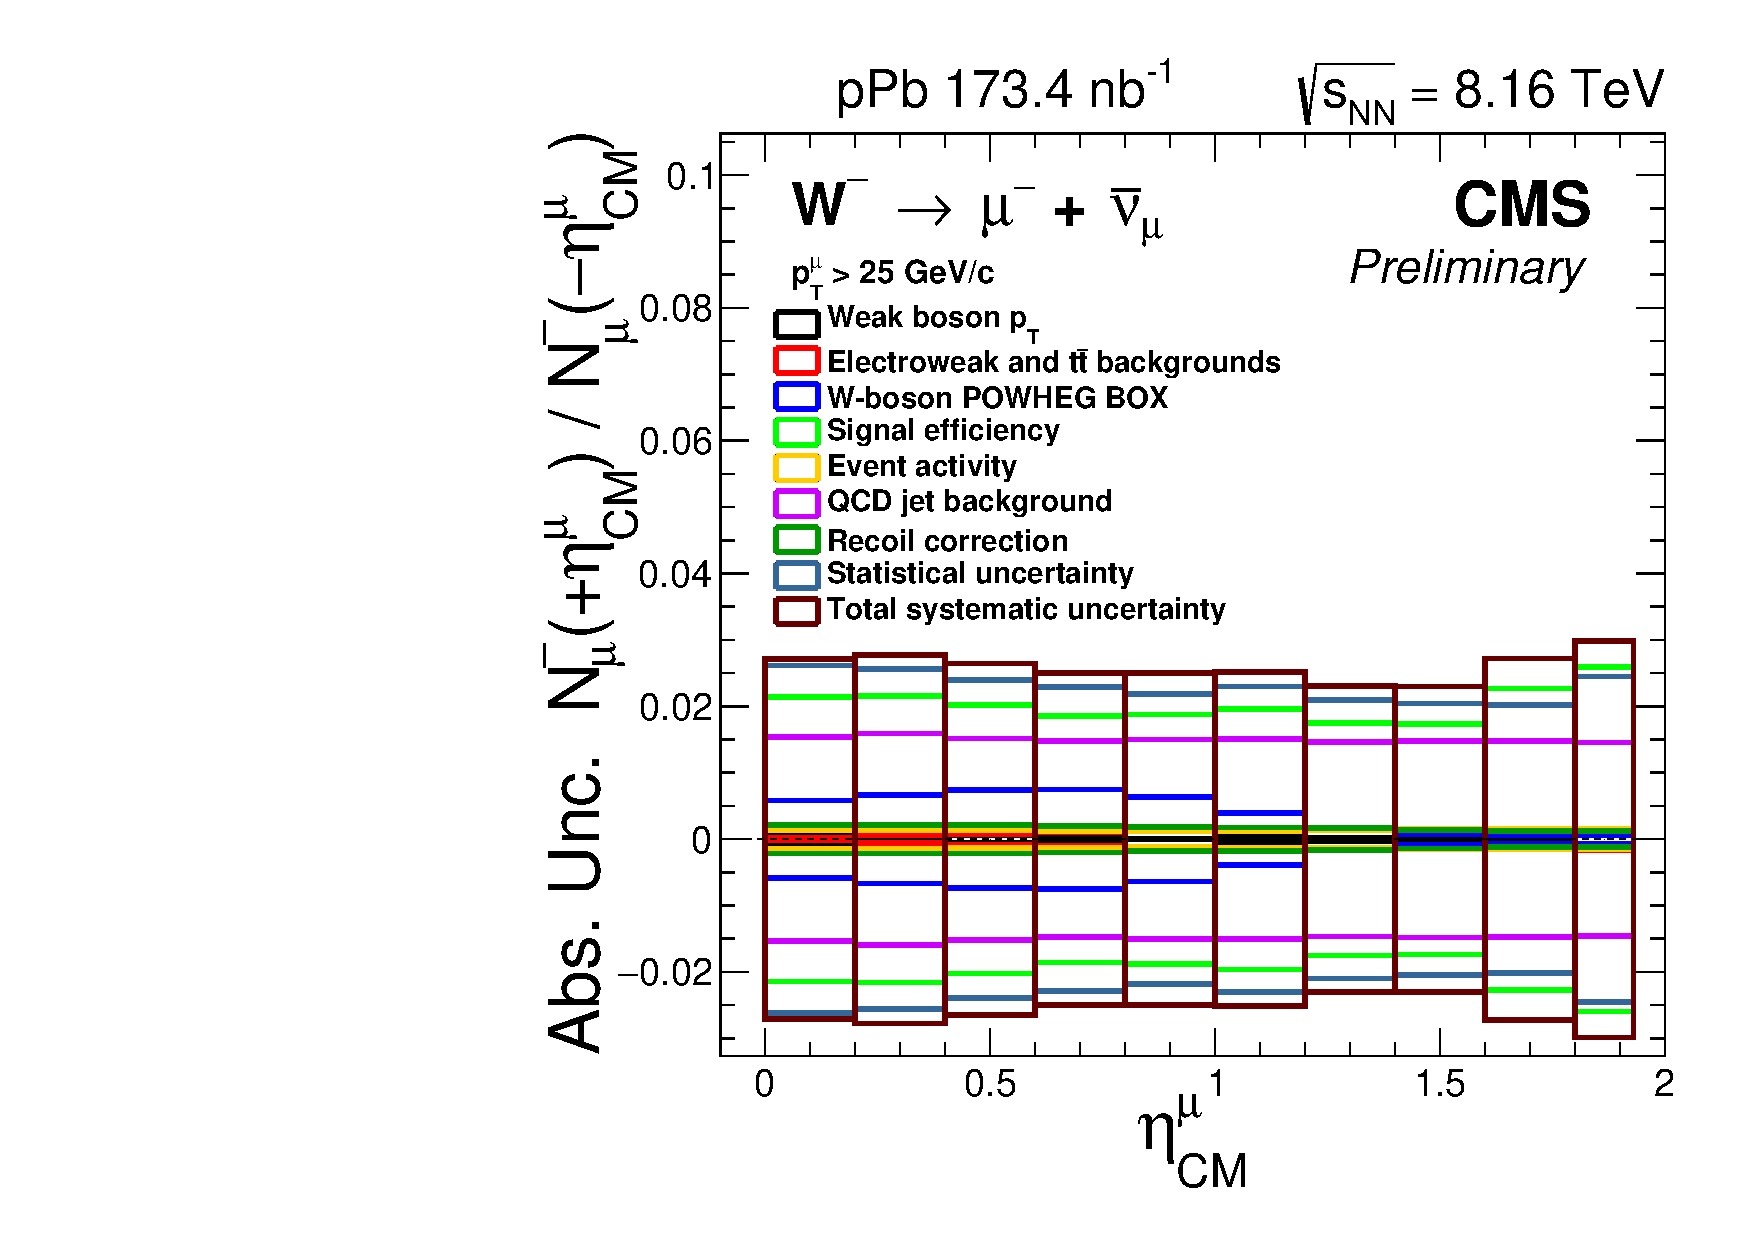
\includegraphics[width=0.45\textwidth]{Figures/WBoson/Analysis/Systematics/gr_WToMuMi_PA_ForwardBackward_Ratio_EffTnP.pdf}
 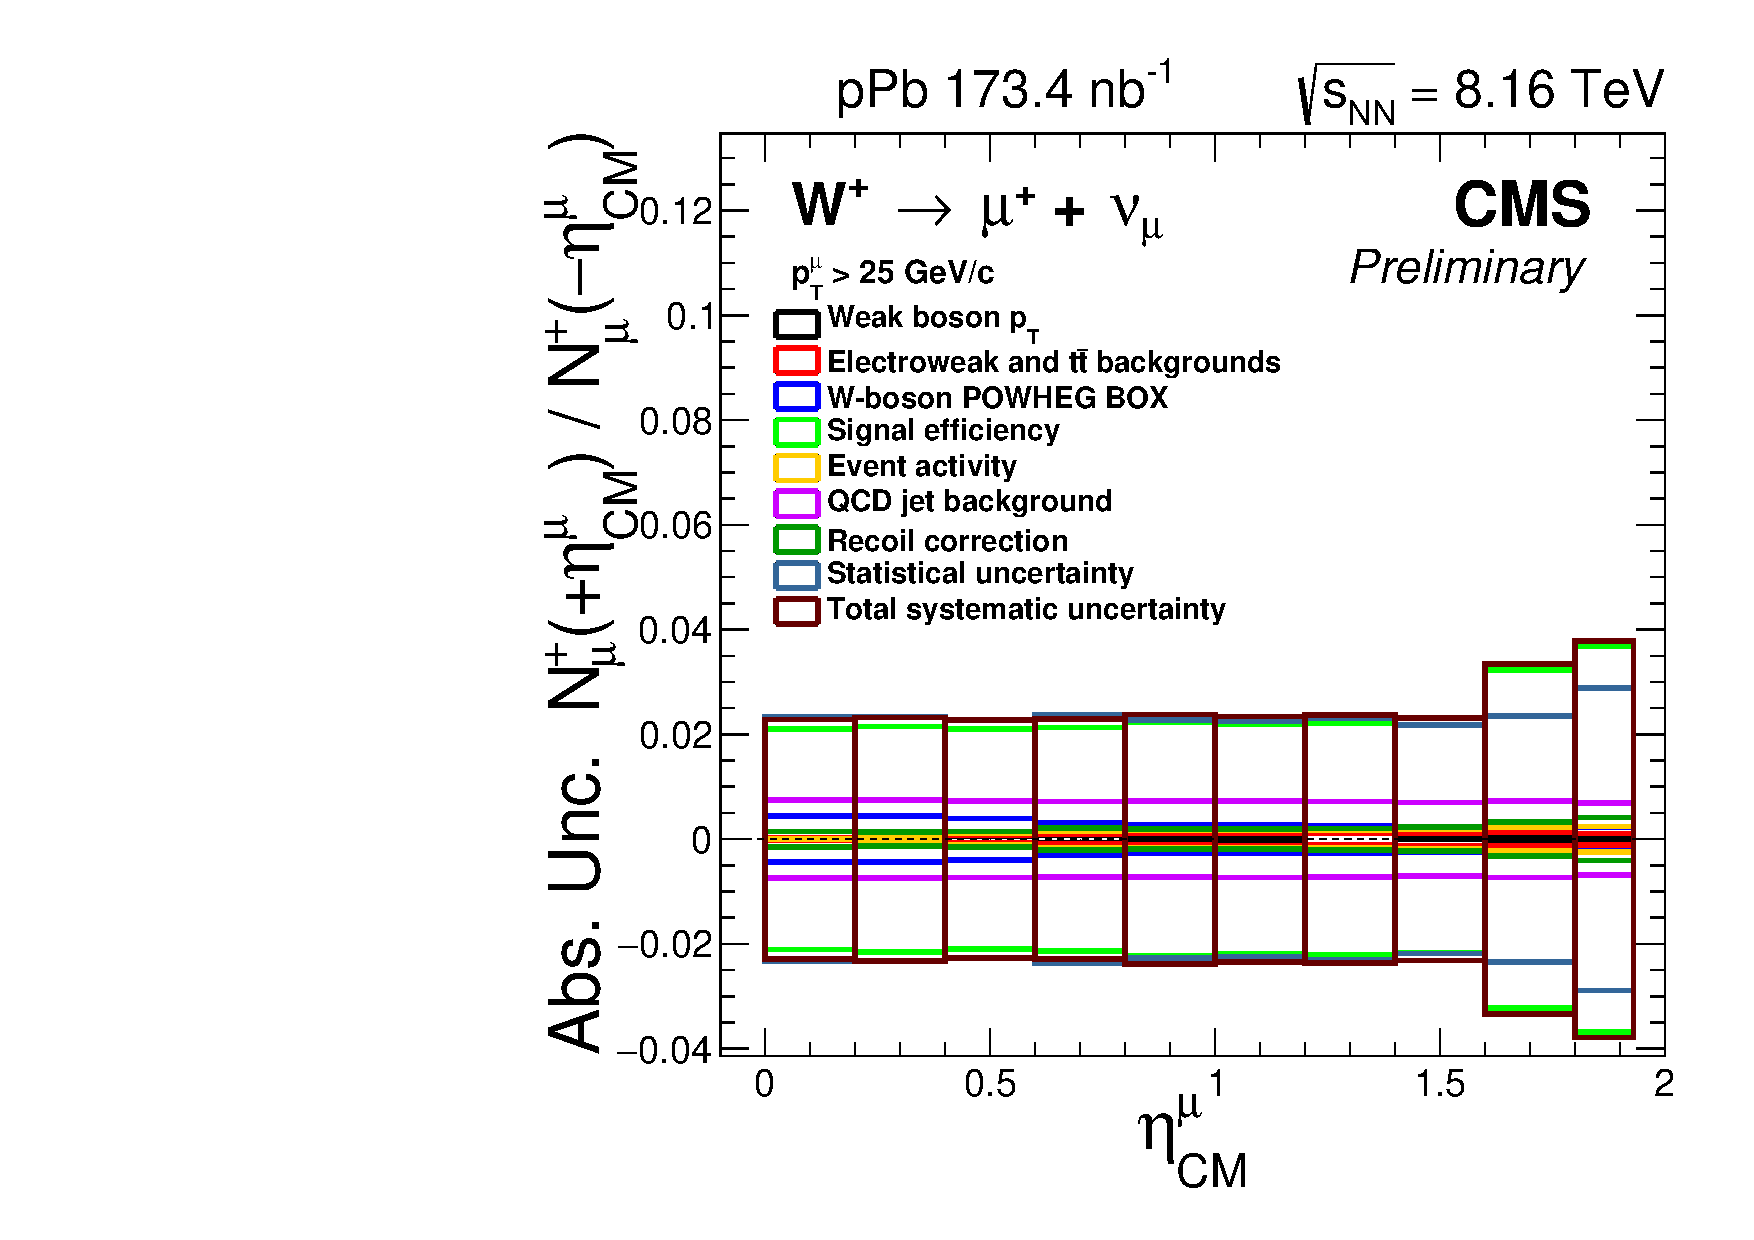
\includegraphics[width=0.45\textwidth]{Figures/WBoson/Analysis/Systematics/gr_WToMuPl_PA_ForwardBackward_Ratio_EffTnP.pdf}
\\
 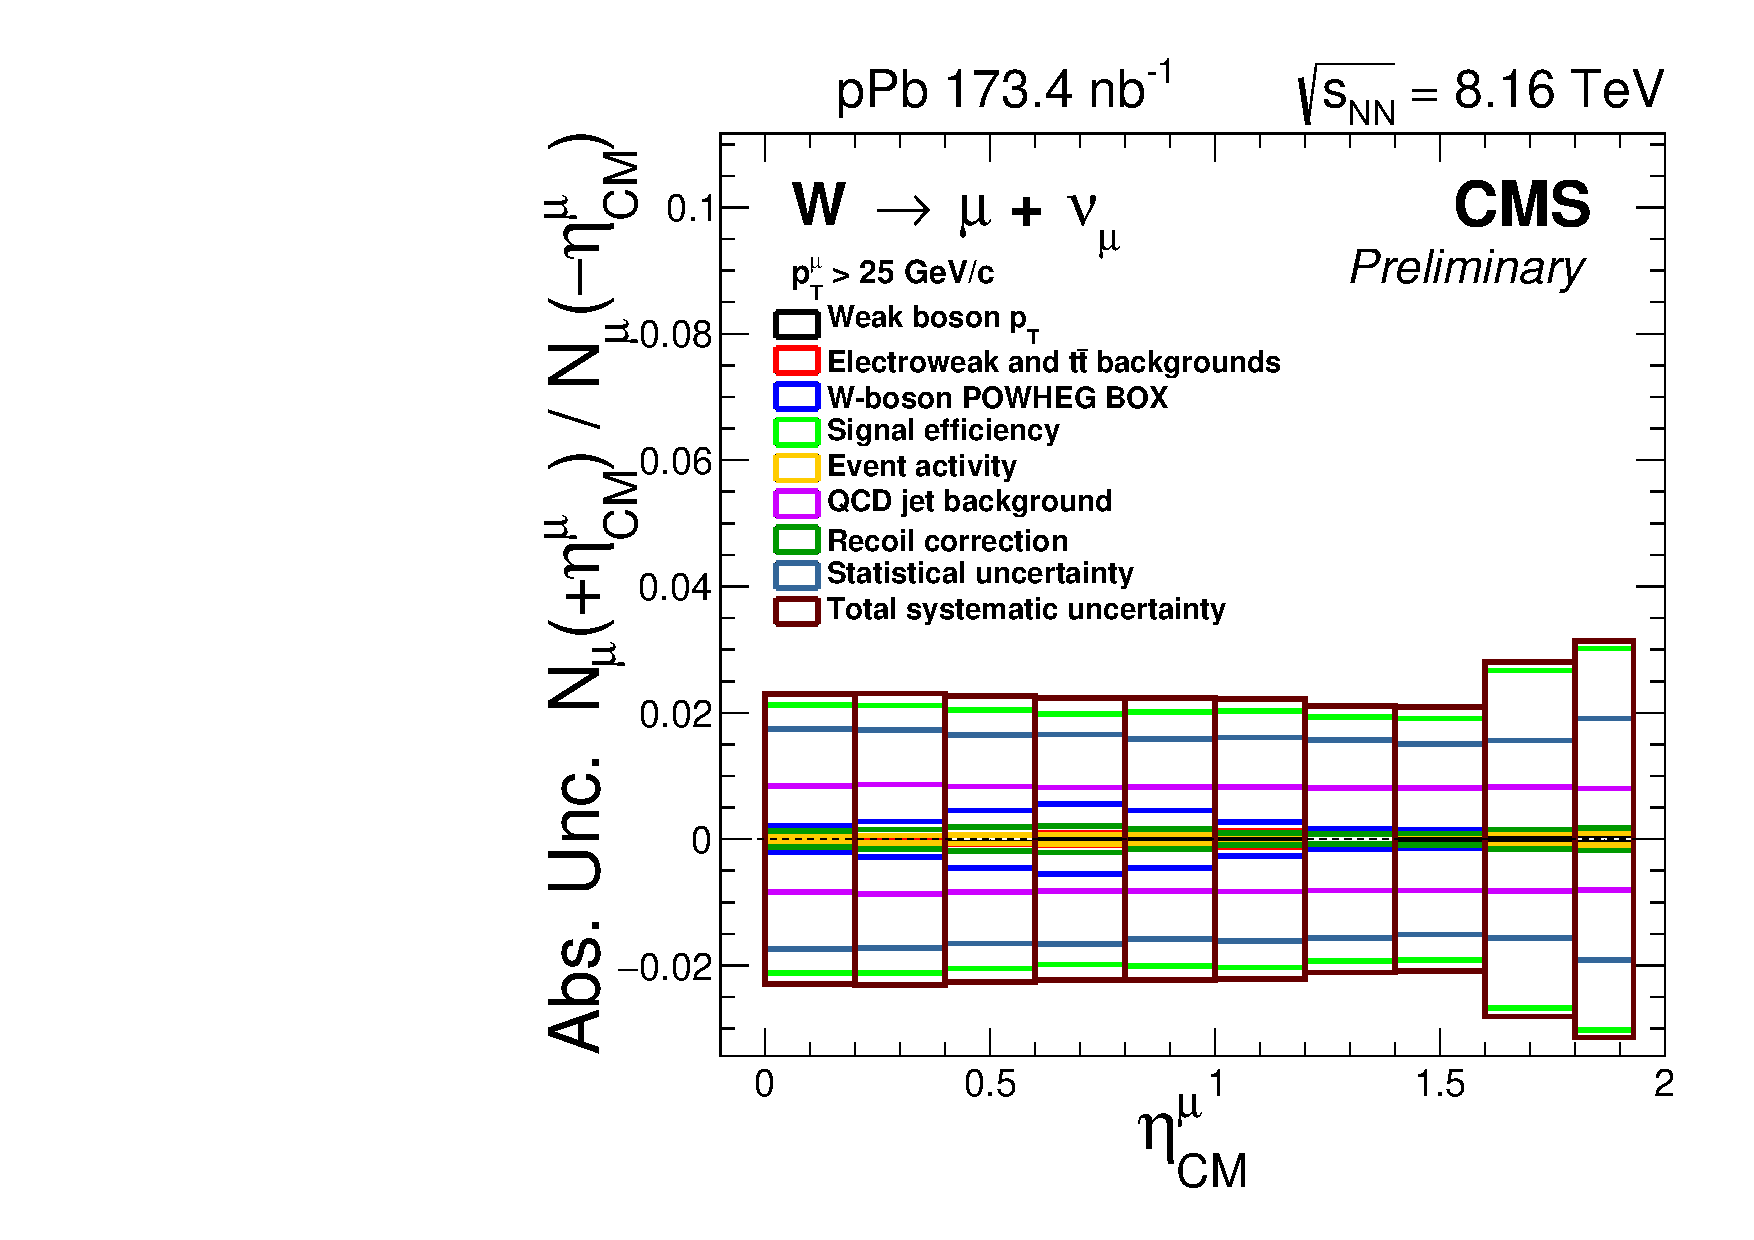
\includegraphics[width=0.45\textwidth]{Figures/WBoson/Analysis/Systematics/gr_WToMuInc_PA_ForwardBackward_Ratio_EffTnP.pdf}
 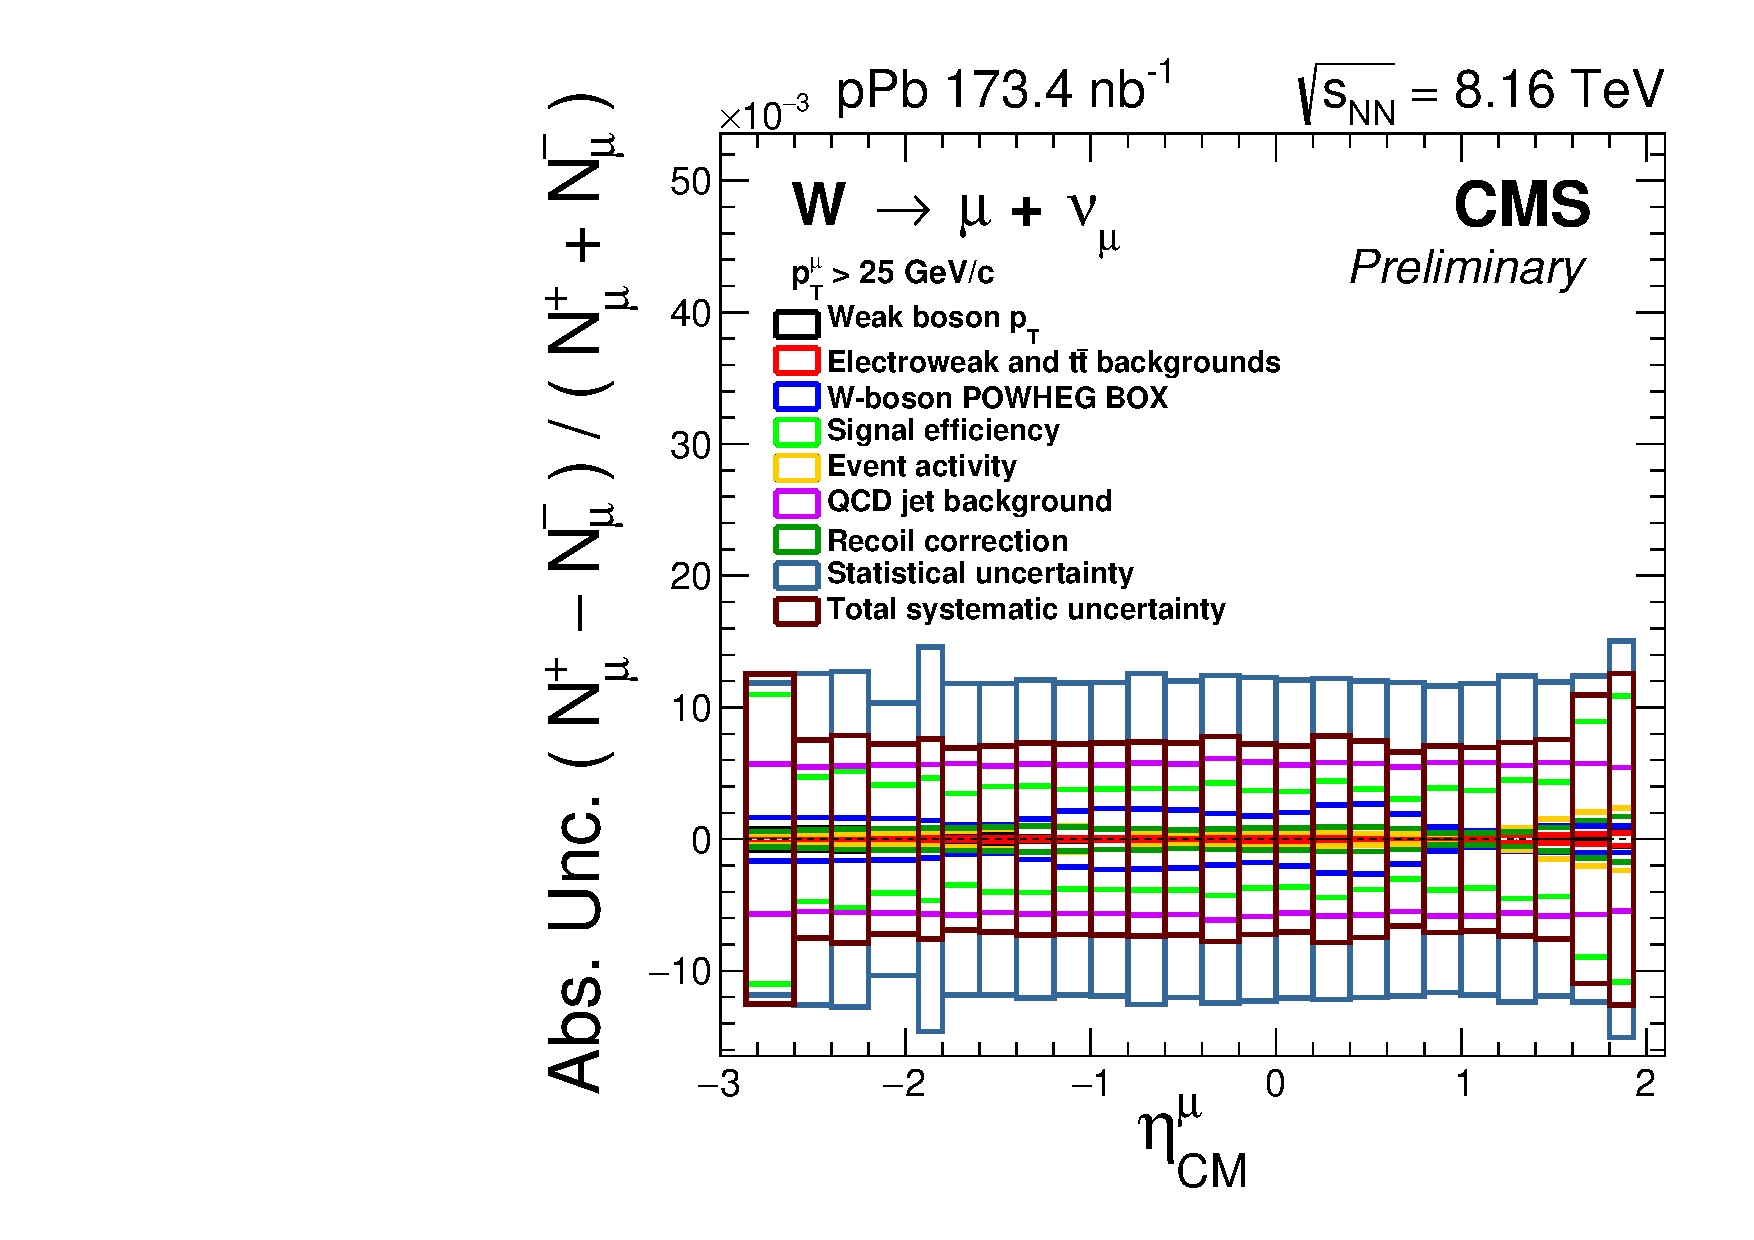
\includegraphics[width=0.45\textwidth]{Figures/WBoson/Analysis/Systematics/gr_WToMuInc_PA_Charge_Asymmetry_EffTnP.pdf}
 \caption{Uncertainty corresponding to each category with respect to \etaCM. The plots are divided as: \WToMuNuMi (top-left) and \WToMuNuPl (top-right) cross sections, \WToMuNuMi (middle-left) and \WToMuNuPl (middle-right) \RFB, and the charge-summed \RFB (bottom-left) and muon charge asymmetry (bottom-right). The uncertainties of the cross sections are relative while for the \RFB and muon charge asymmetry are absolute. The luminosity uncertainty is not included.}
 \label{fig:Summary_Systematics}
\end{figure}


%%------------------------------------------------------------%%
\subsubsection{Covariance matrix}\label{sec:WBoson_Analysis_Systematics_CovarianceMatrix}

The covariance matrices of the \WToMuNu differential cross sections, the forward-backward ratios and the muon charge asymmetry are computed by taking into account the measurements extracted in each \etaMuCM range. In the case of the \WToMuNupm differential cross sections and the \WToMuNupm forward-backward ratios, the matrices are made of 48x48 entries (24 muon \etaMuCM ranges times two muon charge measurements), while for the muon charge asymmetry and the charge-summed forward-backward ratio, only 24x24 entries are considered.

For a given ($i$, $j$) entry of the covariance matrix, the covariance is calculated as the uncertainty in bin $i$ times the uncertainty in bin $j$. If the uncertainty is uncorrelated, the off-diagonal elements are set to zero. The total covariance matrix of each observable is determined by summing the covariance matrix of the statistical uncertainty together with the covariance matrices of all the systematic uncertainties.

The covariance matrix of the statistical uncertainty corresponds to a fully diagonal matrix where each ($i$, $i$) element in the diagonal is the square of the statistical uncertainty of bin $i$. On the other hand, the covariance matrix of each systematic uncertainty is computed by taking into account the bin-to-bin correlations in muon charge and pseudorapidity.

The total correlation matrix of each observable is derived from the total covariance matrix, using the following formula:

\begin{equation}
 \corr\left(i,j\right) = \frac{\cov\left(i,j\right)}{\sqrt{\cov\left(i,i\right)\times\cov\left(j,j\right)}}
\end{equation}

The corresponding correlation matrices are shown in \fig{fig:CorrelationMatrix}. The black lines are used to distinguish the different bins in muon charge, which are ordered in a given plot from top to bottom as: Minus-Minus, Minus-Plus, Plus-Minus and Plus-Plus. The large correlation observed in the \WToMuNu differential cross sections arises from the luminosity uncertainty. On the other hand, the \tnp corrections for muon isolation and identification are applied in wide $|\etaLAB|$ intervals which justify the anti-correlation observed with respect to $\etaCM$ in the muon charge asymmetry.

\begin{figure}[htb!]
 \centering
 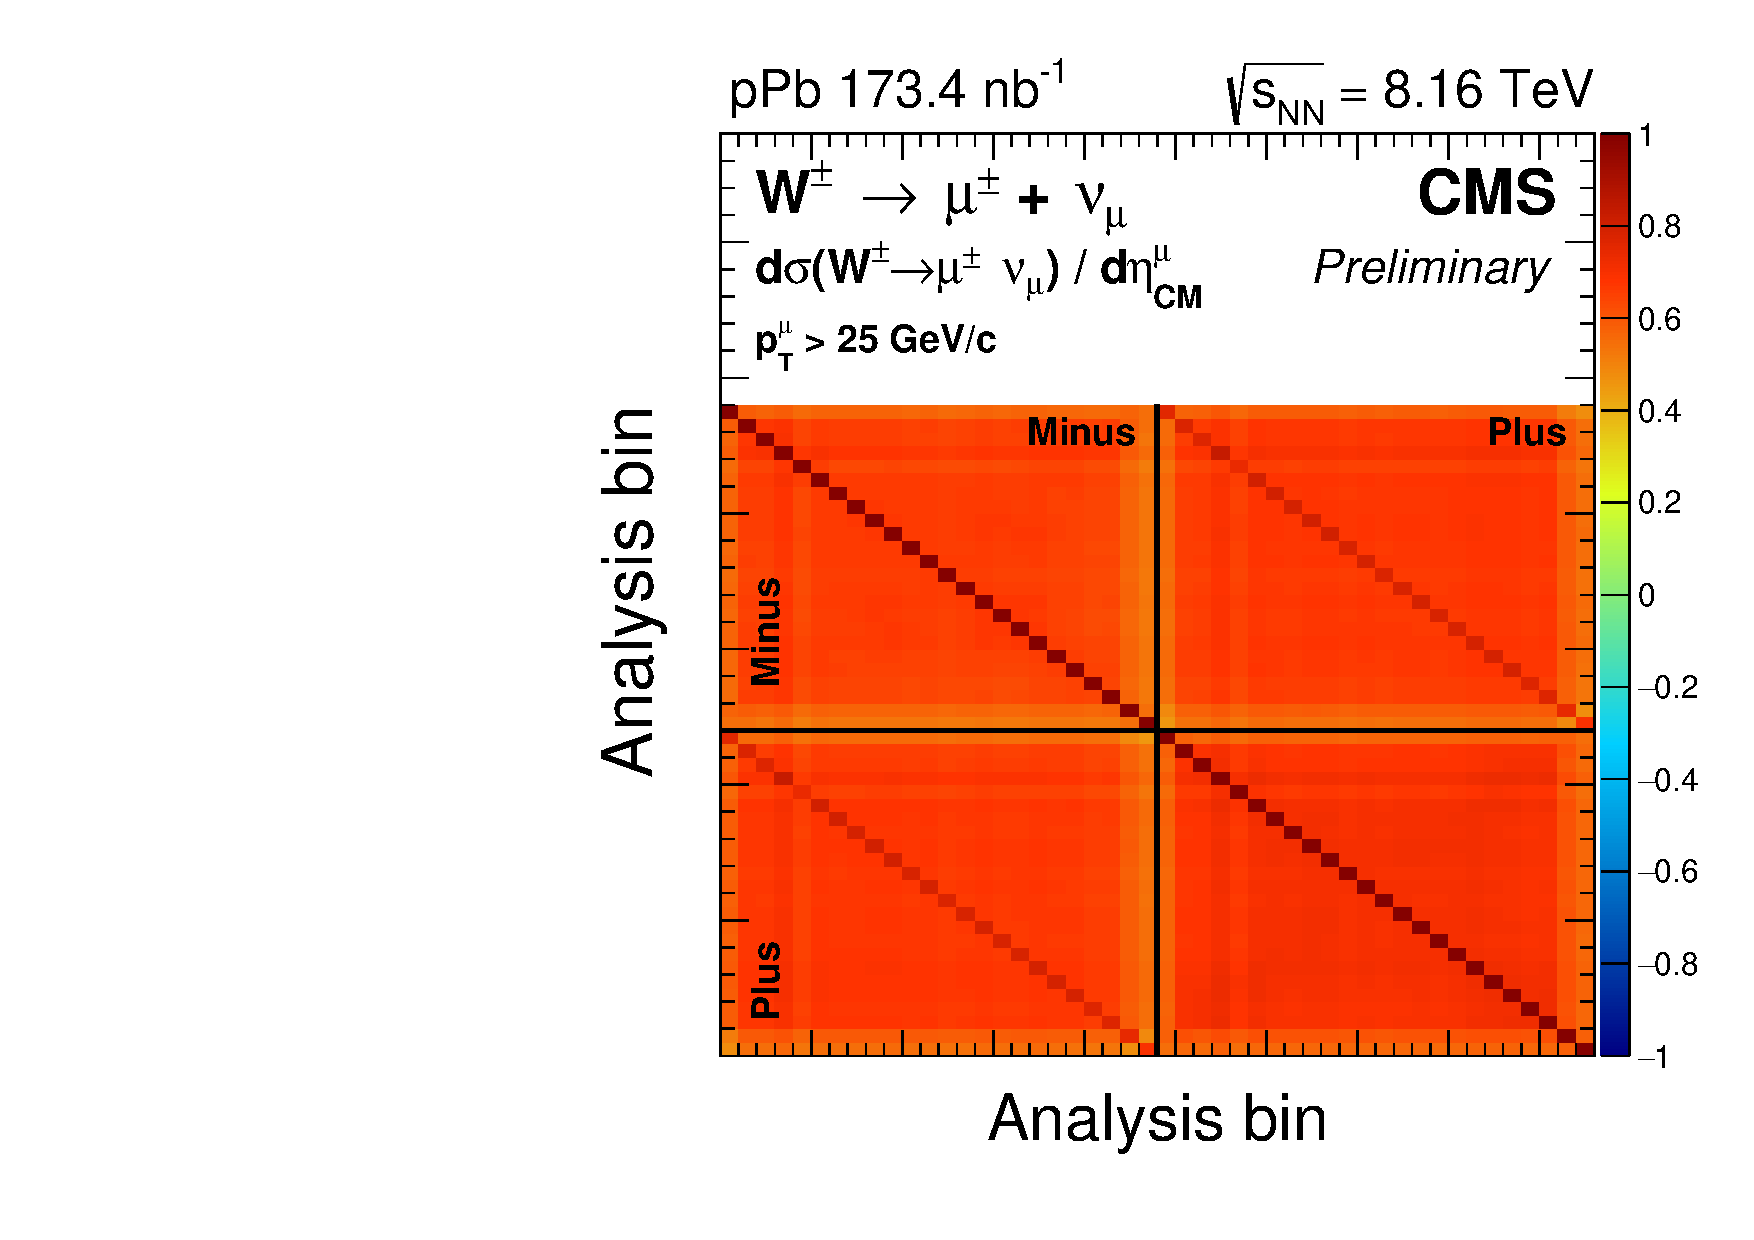
\includegraphics[width=0.45\textwidth]{Figures/WBoson/Analysis/CovarianceMatrix/corMatrix_WToMuPl_PA_Cross_Section_Total_Total.pdf}
 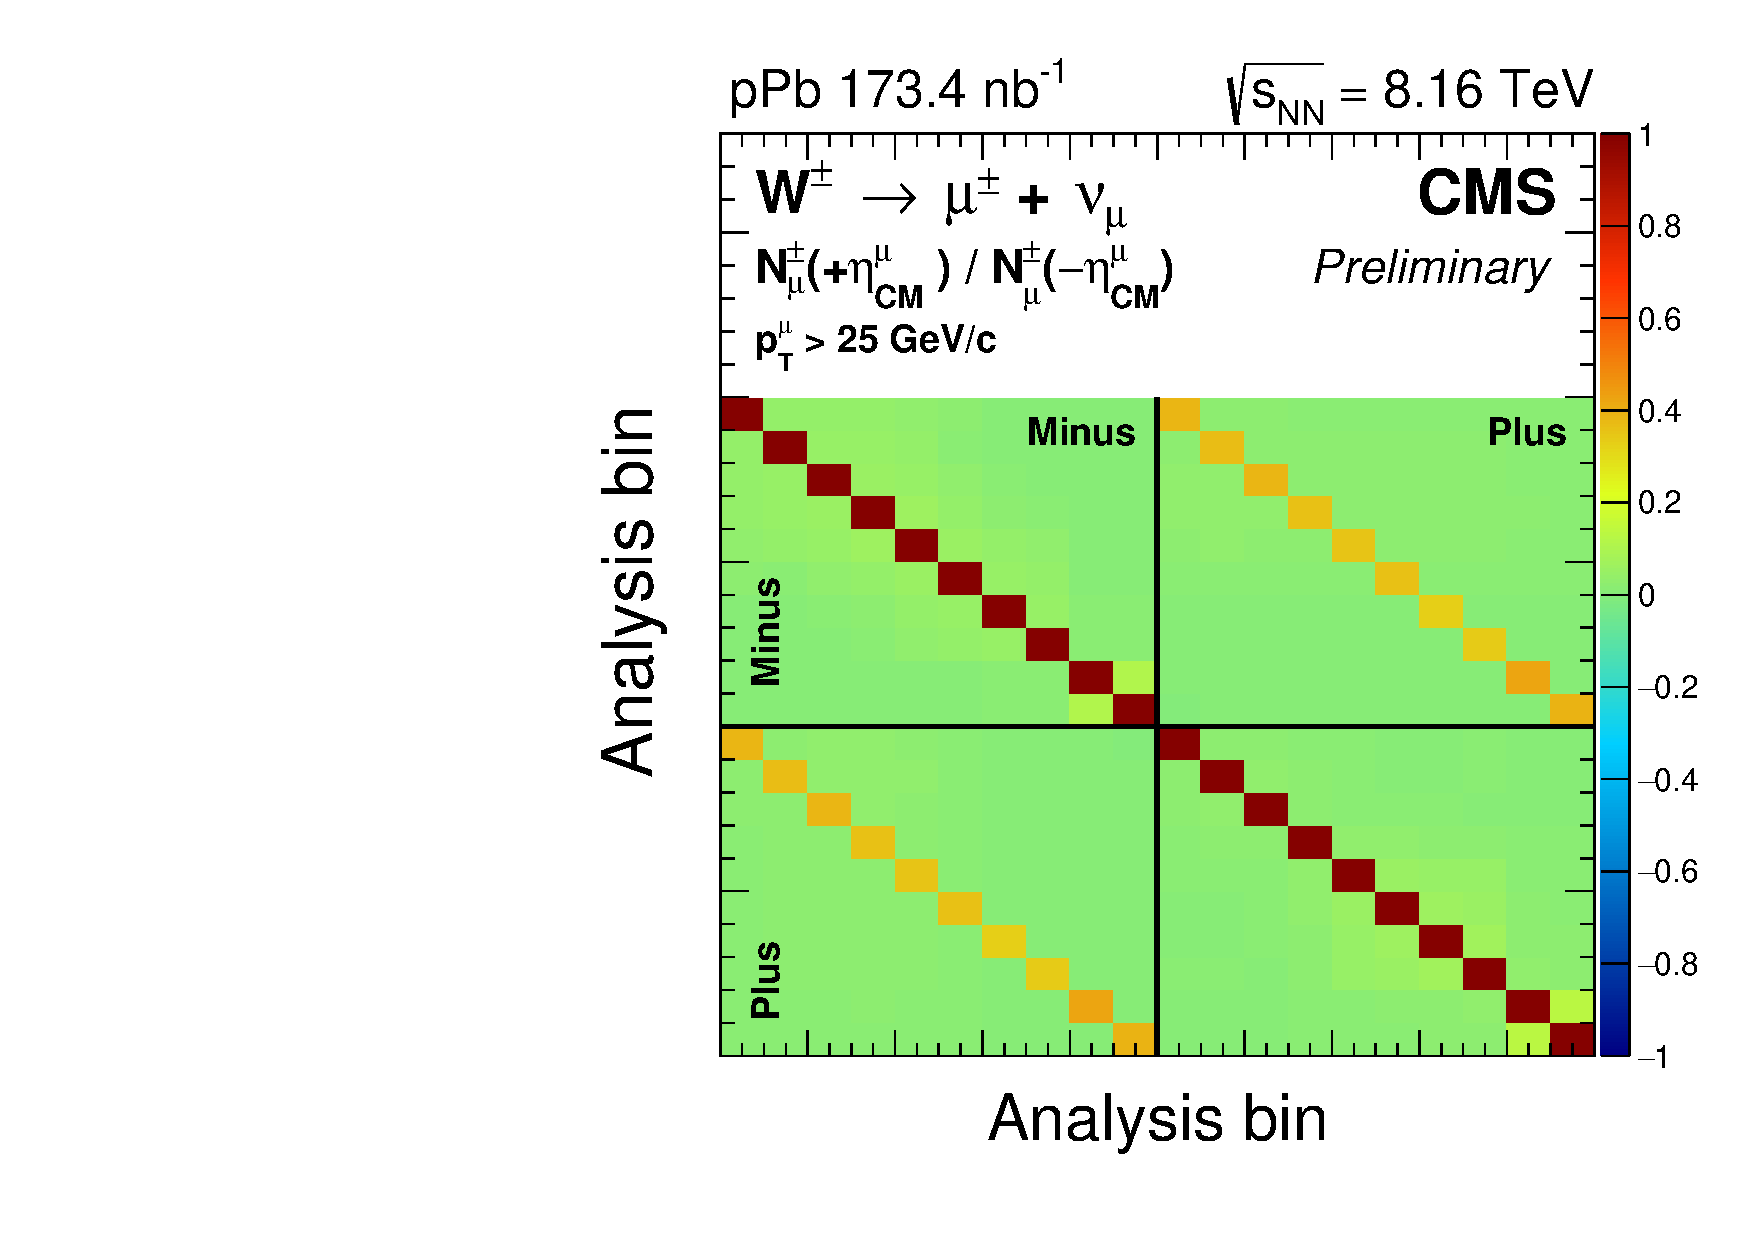
\includegraphics[width=0.45\textwidth]{Figures/WBoson/Analysis/CovarianceMatrix/corMatrix_WToMuPl_PA_ForwardBackward_Ratio_Total_Total.pdf}
%%
 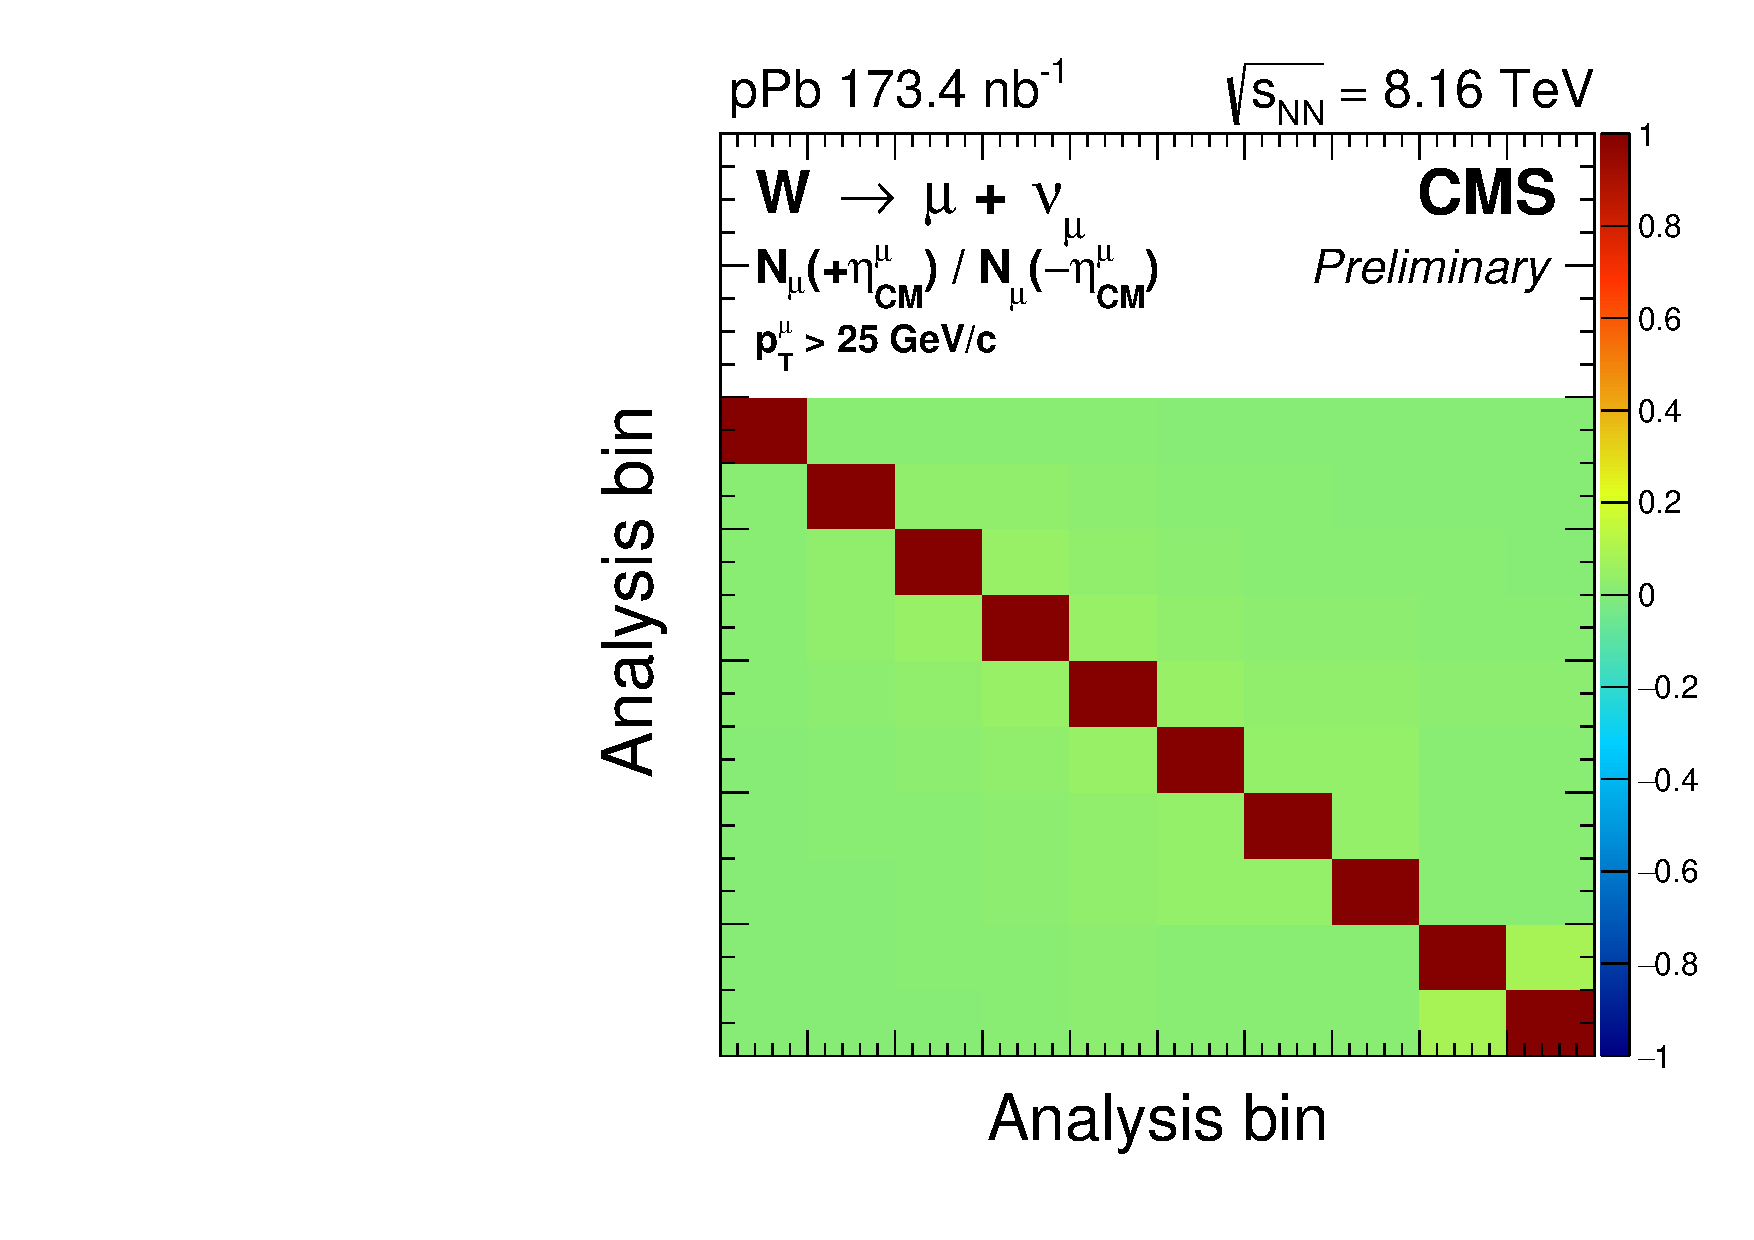
\includegraphics[width=0.45\textwidth]{Figures/WBoson/Analysis/CovarianceMatrix/corMatrix_WToMu_PA_ForwardBackward_Ratio_Total_Total.pdf}
 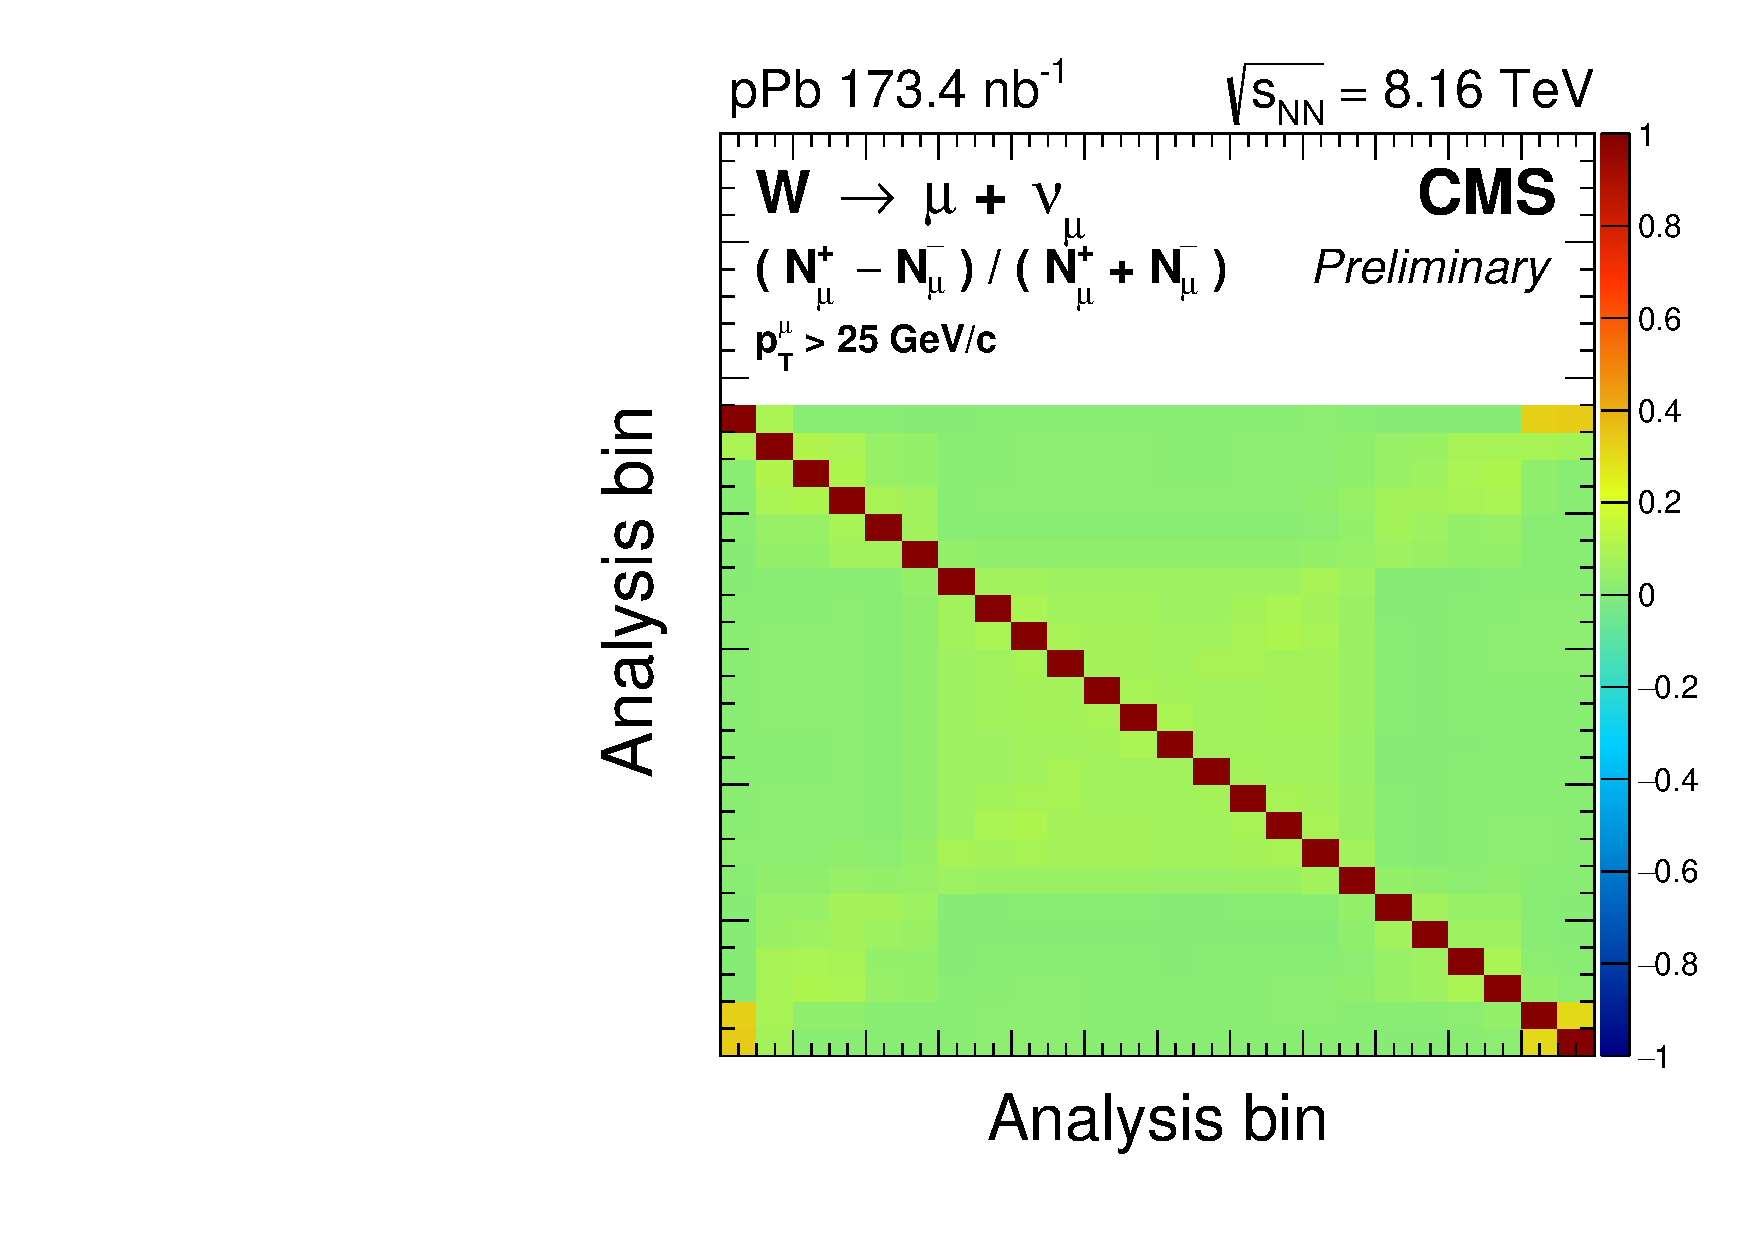
\includegraphics[width=0.45\textwidth]{Figures/WBoson/Analysis/CovarianceMatrix/corMatrix_WToMu_PA_Charge_Asymmetry_Total_Total.pdf}
 \caption{Correlation matrices for: \Wpm cross section (top-left) , \Wpm $R_{FB}$ (top-right) , charge-inclusive $R_{FB}$ (bottom-left) , and charge asymmetry (bottom-right). The lines in the top plots are used to separate the different muon charge bins.}
 \label{fig:CorrelationMatrix}
\end{figure}


% END OF SUBSECTION